% ****** Start of file apssamp.tex ******
%
%   This file is part of the APS files in the REVTeX 4.1 distribution.
%   Version 4.1r of REVTeX, August 2010
%
%   Copyright (c) 2009, 2010 The American Physical Society.
%
%   See the REVTeX 4 README file for restrictions and more information.
%
% TeX'ing this file requires that you have AMS-LaTeX 2.0 installed
% as well as the rest of the prerequisites for REVTeX 4.1
%
% See the REVTeX 4 README file
% It also requires running BibTeX. The commands are as follows:
%
%  1)  latex apssamp.tex
%  2)  bibtex apssamp
%  3)  latex apssamp.tex
%  4)  latex apssamp.tex
%
\documentclass[%
 reprint,
%superscriptaddress,
%groupedaddress,
%unsortedaddress,
%runinaddress,
%frontmatterverbose,
%preprint,
%showpacs,preprintnumbers,
%nofootinbib,
%nobibnotes,
%bibnotes,
 amsmath,amssymb,
 aps,
 norsk,
 booktabs
%pra,
%prb,
%rmp,
%prstab,
%prstper,
%floatfix,
]{revtex4-1}

\usepackage[utf8]{inputenc}
\usepackage[norsk]{babel}
\usepackage{varioref}
\usepackage{graphicx}% Include figure files
\usepackage{enumitem}
\usepackage{dcolumn}% Align table columns on decimal point
\usepackage{bm}% bold math
\usepackage[margin=0.9in]{geometry}
\usepackage[mathlines]{lineno}% Enable numbering of text and display math
%\linenumbers\relax % Commence numbering lines

\usepackage[usenames,dvipsnames,svgnames,table]{xcolor}
\usepackage[colorlinks]{hyperref}
\usepackage{relsize}
%\usepackage{booktabs}
\usepackage{graphicx,verbatim,amsfonts,geometry}
\usepackage{amsmath}
\newcommand*\diff{\mathop{}\!\mathrm{d}}
\newcommand*\Diff[1]{\mathop{}\!\mathrm{d^#1}}
\usepackage{ulem}
\usepackage{amssymb}
\usepackage{multirow}
\usepackage{soul}
\usepackage{dsfont}
% allows for temporary adjustment of side margins
\usepackage{chngpage}
% just makes the table prettier (see \toprule, \bottomrule, etc. commands below)
\usepackage{booktabs}

\usepackage{commath}
\usepackage{wrapfig}
\usepackage[free-standing-units=true]{siunitx}
\DeclareSIUnit\year{yr}
\usepackage{gensymb}
\newcommand{\ROM}[1]{%
  \textup{\uppercase\expandafter{\romannumeral#1}}%
}
\usepackage{physics}
\usepackage{caption}
\usepackage{bm}
\usepackage{gensymb}

\makeatletter
\newcounter{elimination@steps}
\newcolumntype{R}[1]{>{\raggedleft\arraybackslash$}p{#1}<{$}}
\def\elimination@num@rights{}
\def\elimination@num@variables{}
\def\elimination@col@width{}
\newenvironment{elimination}[4][0]
{
    \setcounter{elimination@steps}{0}
    \def\elimination@num@rights{#1}
    \def\elimination@num@variables{#2}
    \def\elimination@col@width{#3}
    \renewcommand{\arraystretch}{#4}
    \start@align\@ne\st@rredtrue\m@ne
}
{
    \endalign
    \ignorespacesafterend
}
\newcommand{\eliminationstep}[2]
{
    \ifnum\value{elimination@steps}>0\sim\quad\fi
    \left[
        \ifnum\elimination@num@rights>0
            \begin{array}
            {@{}*{\elimination@num@variables}{R{\elimination@col@width}}
            |@{}*{\elimination@num@rights}{R{\elimination@col@width}}}
        \else
            \begin{array}
            {@{}*{\elimination@num@variables}{R{\elimination@col@width}}}
        \fi
            #1
        \end{array}
    \right]
    &
    \begin{array}{l}
        #2
    \end{array}
    \addtocounter{elimination@steps}{1}
}
\makeatother
% Document formatting
\setlength{\parindent}{0mm}
\setlength{\parskip}{1.5mm}

\begin{document}

\title{Solcelle}
\author{\textsc{Ivar Svalheim Haugerud}}
\affiliation{ Universitetet i Oslo}
\date{\today}

\begin{abstract}
Hva er effektiviteten til en solcelle? La oss finne ut av det.
\end{abstract}

\pacs{Valid PACS appear here}% PACS, the Physics and Astronomy
                             % Classification Scheme.
%\keywords{Suggested keywords}%Use showkeys class option if keyword
                              %display desired
\maketitle

%\tableofcontents
\section{Introduksjon}
Mennesker har i århundrer prøvd å lage en evighetsmaskin. Fysikkens lover har vist at dette er umulig, energi er alltid bevart. Derimot kan en argumentere for at mennesker har klart å lage en evighetsmaskin ved solceller. Hvert sekund blir hver kvadratmeter av atmosfæren vår bestrålt med en energi på $\SI{1355}{\joule}$ \cite{oppgave}. Denne energien har truffet planeten i flere miliarder av år, og solen kommer til å fortsette å tilføre denne energien i all overskuelig fremtid. Solceller har en ufattelig stor, og tilnærmet evigvarende, energikilde å tappe energi fra. Og det er med dette i tankene at en kan argumentere for at evighetsmaskinen finnes, solcellen. Det er kanskje derfor bruk av solceller har skutt til himmels det siste tiåret \cite{oppgave}.\par
Selv om vi klarer å utnytte energien fra sola vår, er man ikke fornøyd med andel av energien man får bruk for. Av det som treffer atmosfæren vår er det $\SI{950}{\watt\per\meter^2}$ som når fram til jordoverflaten på en klar dag. Resten av energien blir absorbert eller reflektert i atmosfæren. Komersielle solceller klarer å utnytte mellom $15-22\%$ av energien som treffer jordoverflaten. Forskning innenfor solceller prøver å gjøre det rimeligere å produsere, og øke andelen av energien man får utnyttet. Vi ønsker derfor i dette eksperimentet å finne den maksimale effekten til en solcelle, og forstå hvordan man klarer å maksimere effekten. For å gjøre dette blir det gjennomført målinger av solceller, bestrålt av et kontrollert lys, i forskjellige situasjoner. Ved å gjøre målinger på strømmen i kretsen, og spenningen over solcellen kan vi finne strøm-spenning karakteristikken til solcellen. Fra disse målingene finner man den maksimale effekten en kan oppnå. Solcellene ble koblet i serie og parallell med hverandre for å se nærmere på effekten dette har på strømen og spenningen produsert av solcellen. Disse målingene skal gjøres mens solcellen er fullstendig belyst, delvis belyst og ubelyst for å forstå hvordan solceller oppfører seg under forskjellige omgivelser.
\section{Teori}
\subsection{Kretsteori}
I starten av det forrige århundet fant man uttrykket for energien til et foton. Dette uttryket viser at energien $E$ til et foton er propsjonal med frekvensen, $\nu$, til fotonet
\begin{equation}
  E = h\nu = \frac{hc}{\lambda} \label{einstein},
\end{equation}hvor $h$ er Plancks konstant, $c$ er lyshastigheten, og $\lambda$ er bølgelengden til fotonet. Denne relasjonen ble påvist av Einstein i 1905 gjennom målinger på den fotoelektriske effekt. Som den fotoelektriske effekt kommer solcellen til å være koblet i en krets med forskjellige komponenter. Den viktigste relasjonen vi kommer til å bruke er Ohms lov
\begin{equation}
  V = RI,
\end{equation}som sier at spenningsfallet $V$ er gitt av produktet mellom strømmen $I$ og resistansen $R$. Dette kan brukes for å finne effekttapet, $P$, til en komponent er gitt av produktet mellom spenningsfallet $V$ over komponenten og strømmen som går gjennom den
\begin{equation}
  P = VI = RI^2 = \frac{V^2}{R} \label{effekt1}.
\end{equation}For å få lage den beste mulige solcelle burde effekten $P$ være så stor som mulig. Vi kommer derfor til å trenge noen viktige relasjoner for den maksimale effektiviteten $P_{max}$. Under eksperimentet kommer vi til å gjøre målinger for å finne strøm-spenningskarkateristikkentil solcellen. Vi kommer derfor til å finne solcellens spenning med uendelig stor belastning, det vil si \textit{open circuit}, $V_{oc}$. Og hvilken strøm som går i solcellen når kretsen er kortsluttet, det vil si \textit{short circuit}, $I_{sc}$. Det viser seg at forholdet mellom den maksimale effekten og produktet av $V_{oc}$ og $I_{sc}$ er konstant, og har fått navnet \textit{fill factor}.
\begin{equation}
  \frac{P_{max}}{V_{oc}I_{sc}} = FF. \label{ff}
\end{equation}Dette er en nyttig relasjon når vi skal studere forholdet mellom effekter. Årsaken til dette er et fill factor er en karakteristikk av solcellen, og er ikke avhengig av eksterne forhold. Siden fill factor er tilnærmet lik konstant kan vi finne forholdet mellom to effekter ved å bruke definisjonen av fill factor
\begin{equation}
  \frac{\left(P_{max}\right)_1}{\left(P_{max}\right)_2} \approx \frac{\left(V_{oc}I_{sc}\right)_1}{\left(V_{oc}I_{sc}\right)_2}. \label{maxP}
\end{equation}Hvor måling $1$ og måling $2$ kan henvise til f.eks målinger av samme solcelle, men emd forskjellig belysning.\\For å beregne effektiviteten til solcellen blir det brukt et solarimeter under eksperimentet. Solarimeteret har en kalibreringskonstant $a$ som gjør det mulig å beregne den bestrålte effekten på solcellen. Den bestrålte effekten er gitt av produktet mellom spenningen over solarimeteret $V_s$ og arealet $A$ av solcellen, som må divideres på kalibreringskonstanten $a$
\begin{equation}
  P_{inn} = \frac{V_sA}{a} \label{kalibrering}.
\end{equation}
Ved å vite $P_{inn}$ kan man beregne effektiviteten ved å sammenlikne denne verdien med den maksimale effekten i kretsen. Dette gjøres ved
\begin{equation}
  \text{effekt} = \frac{P_{max}}{P_{inn}}\cdot 100\%\label{effekt}
\end{equation}
\subsection{Halvledere og solceller}
De fleste solceller er laget av halvledermateriale, for å forstå solceller må vi derfor forstå halvledere. Halvledere fungerer på grunn av kvanatiserte energinivåer til atomer. Elektroner i atomer oppbevarer seg på elektronskall som tilsvarer kvantetallet deres, $n\in\mathbb{N}$. For hvert energinivå er det oppdelt i underskall som blir bestemt av det azimutale kvantetallet $l \in \mathbb{N} < n$. Denne elektronkonfigurasjonen er forskjellig for forskjellig atomer, og bestemmer de kjemiske og fysiske prosessene til atomet.\\
Bindinger mellom atomer bestemmes av elektronene i de ytterste skallene, elektronene med størst $n$, som kalles valenselektronene. Ved å tilføre elektroner energi til elektronene vil de eksiteres, de flytter seg til et høyere skall. Siden energinivåene er kvantiserte vil forflytningen være kvantisert. For like atomer er disse energinivåene identiske, men når vi har flere identiske atomer sammen oppstår det nye effekter, \textit{more is different}. De originiale energinivåene splittes opp til flere forskjellige energinivåer. Antall forskjellige energinivåer øker med antall atomer, og er det nok atomer tilstede vil det bli dannet et kontinuerlig energibånd. Energibåndet som dannes av valenselektroner kalles valensbåndet. Er valensbåndet fullt av andre elektroner kan ikke elektronene flytte på seg, på grunn av Paulis eksklusjonsprinsipp, for å danne strøm i valensbåndet. Det blir først mulig å danne strøm hvis elektronene blir eksitert til det neste ikke-okkuperte energibåndet, som er over valensbåndet, dette båndet kalles ledningsbåndet. For silisium, som vi bruker i dette eksperimentet, og andre halvledere, er det et energiområde mellom valensbåndet og ledningsbåndet hvor elektronet ikke kan ha en energitilstand. Dette området kalles båndgapet, for silisium er størrelsen på båndgapet $\SI{1.12}{\electronvolt}$.\par
Halvledere kan beholde krystallstrukturen sin, og forbedre sin elektriske ledningsevne, ved å bli dopet av fremmedatomet. Doping innebærer at man erstatter en svært liten andel ($1/10^6$) av silisiumatomene med andre atomer. For at fremmedatomet skal binde seg til silisiumsgitteret trenger det fire valenselektroner. Arsen har fem valenselektroner, som gjør at det siste valenselektronet blir svakt bundet til arsen-atomet. Dette gjør at det lett kan binde seg til nabo silisium-atomet. Elektronet vil derfor fortsette å kunne bevege seg fra atom til atom inne i krystallen. Siden vi har økt antall elektroner kalles dette $n$-doping, $n$ for negativ. Ved å dope silisium med bor-atomer, som har tre valenselektroner, vil det danne en vandrene hull-strøm. Siden vi har redusert antall elektroner kalles dette $p$-doping, $p$ for positiv.\\
Grensesjiktet mellom to halvledere, der den ene er $n$-dopet og den andre er $p$-dopet, kalles for en $pn$-overgang. I dette området, \textit{overgangssonen}, vil noen elektroner for den $n$-dopede halvlederen fylle hullene i den $p$-dopede halvlederen. Denne forflyningen av ladning fører til ladde ioner på hver sode av overgangssonen. Dette gjør at $p$-siden blir netto negativt ladd, og $n$-siden blir netto positivt ladd. Denne ladningsforskjellen mellom de to områdene vil dannet et elektrisk felt fra $n$-type til $p$-type området. Dette feltet vil hindre flere elektroner fra å bevege seg over overgangssonen.\\
Vi har beskrevet hvordan halvledere virker, men ikke hvordan dette er relatert til solceller og lys. For å  forstå dette må vi se nøyere på overgangssonen til silisiumatomer.
%Ladningsforskjellen mellom de to områdene skaper et elektrisk felt som gjør at ladningene ikke klarer å flytte seg over, de har ikke nok energi.
Får ett elektronen tilført energi, ved å absorbere et foton, kan det løsnes fra kjernen og bevege seg fritt i krystallen. Mest sansnylig vil elektronet binne seg med det atomet det ble løsrevet fra, og vi er like langt. Er elektronet i overgangssonen vil retningen på det elektriske feltet gjøre at elektronene blir dratt over til $n$-området, og hullet i retning $p$-området. Spenningsforskjellen har separert elektronet fra hullet. Nå er det et atom på $p$-siden av overgangssonen som har mistet et elektron. Dette hullet kommer til å bli fylt av et annet elektron. Som tiden går vil $p$-området få et overskudd av hull, og $n$-området et overskudd av elektroner. Dette endrer på spenningsforskjell mellom områdene. Nå er det $p$-siden som blir positivt ladd, og $n$-siden blir negativt ladd. Dette gjør at den tidligere spenningsforskjellen avtar, helt til det ikke er noen ladningsforskjell på de to områdene. Dette fører til at det slutter å være transport av elektroner og hull i overgangssonen. Har nå solcellen blitt ubrukelig? Nei, ved å koble $p$-området med $n$-området ved hjelp av en ytre ledning vil elektroner fra $n$-området strømme til hullene i $p$-området. Dette vil gjør at feltstyrken opprettholdes, og prosessen kan gjentas. Strømmen vil fortsette å gå, så lenge lys treffer solcellen.\par
Ikke alt lys vil klare å løsrive elektroner fra atomet. For silisium er energien som trengs $\SI{1.12}{\electronvolt}$. Ved å bruke relasjonen mellom energi og bølgelengde\eqref{einstein} finner vi at det kreves en bølgelengde mindre enn $\SI{1100}{\nano\meter}$ for å løsrive et elektron for å danne et elektron-hull par. Derfor vil alt lys med bølgelengde lengere enn $\SI{1100}{\nano\meter}$ ikke føre til noe strøm i solcellen. Spenningen i solcelle kretsen vil aldri kunne bli større enn energien som kreves å løserive et elektron, per elektron, $V<E/e$. For silisium vil dette bety at spenningen solcellen lager vil alltid være mindre enn $\SI{1.12}{\volt}$. En så lav spenning ville ikke klart å lade opp de fleste batterier for pratktisk nytte. Det er derfor ønskelig å endre på kretsen slik at det kan enten bli høyere spenning, eller høyere strøm i kretsen. For å få høyere spenning kan man koble flere enkeltsolceller i serie, ønskes det høyere strøm kobles det flere enkeltsolceller i parallell. Dette skal vi se nærmere på under eksperimentet.
\section{Eksperimentelt}
Under hele eksperimentet kommer vi til å ha en solcelle i en fast avstand fra en lyskilde. Solcellen plasseren i et stativ på en optisk benk sammen med en lysbildeprosjektor. Avstanden mellom den lyskilden og solcellen er valgt slik at solcellene vi kommer til å bruke under eksperimentet kommer til å være fullstendig belyst. Eksperimentet foregår i ett mørkt rom for å kontrollere belysningen av solcellen.\\
\subsection{Strøm-spenningskarkateristikk}
Vi ønsker å måle strøm-spenningkarakteristikken for en belyst solcelle. Først skal vi finne karakteristikken med en ytre spenningskilde i kretsen, og senere uten en spenningskilde i kretsen.
\subsubsection{Med ytre spenningskilde}
For å finne strøm-spenningkarakteristikken med en ytre spenningskilde blir solcellen koblet i en krets sammen en varierende motstand, en spenningskilde på $5$ volt og to voltmetere. Kretsen er vist i figur \vref{krets1}. For å finne strøm-spenningkarakteristikken må vi måle spenningsfallet over solcellen, og strømmen som går gjennom solcellen. Spenningsfallet over solcellen blir målt av voltmeteret $V$ i figur \vref{krets1}, og strømmen i kretsen blir beregnet fra spenningsfallet over resistansen $R_L$, som vi leser av voltmeteret $V_L$. Under målingene varierer vi størrelsen på motstanden i kretsen, og gjør flere målinger for hver verdi av resistansen, for å begrense usikkerheten i målingene. Vi forventer et knekkpunkt i forholdet mellom strøm og spenning, og vi velger derfor verdier av resistansen slik at vi får mange målinger rundt knekkpunktet. Siden vi ønsker å måle strøm-spenningkarakteristikken både i lederretning (hullstrøm), og i sperreretning (negativ strøm), snur vi polariteten på spenningskilden når vi er fornøyd med målingene i lederretning, og gjentar prosessen.
\begin{figure}[h!]
  \centering
  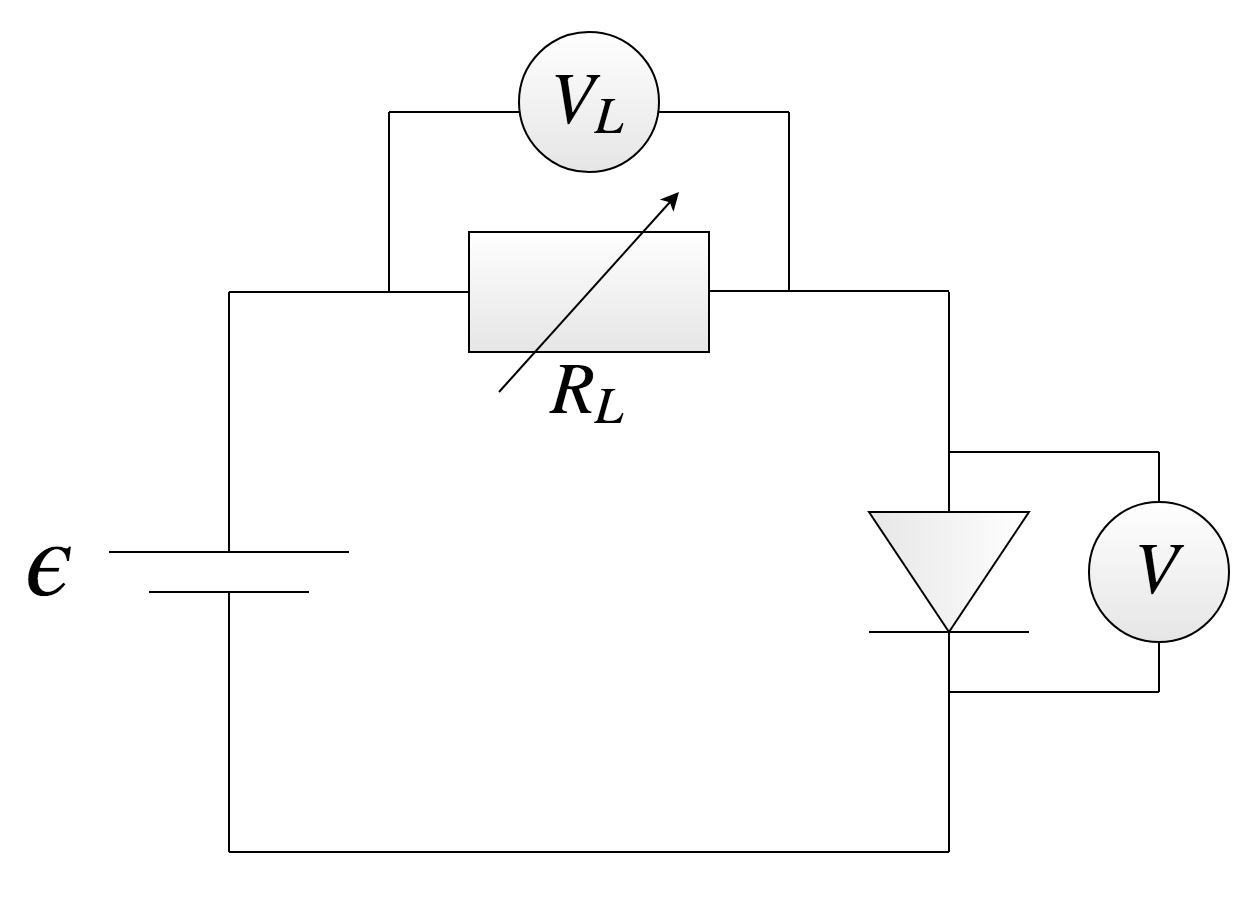
\includegraphics[scale=0.15]{krets1.png}
  \caption{Krets for å måle strøm-spenning karakteristikken til solcellen, med en ytre påtrykket spenning $\epsilon$.}
  \label{krets1}
\end{figure}
\subsubsection{Uten ytre spenningskilde}
Vi ønsker nå å måle strøm-spenningskarkateristikken uten en ytre spenningskilde. Nå skal den eneste spenningskilden i kretsen være solcellen selv. For denne målingen bruker vi kretsen vist i figur \vref{krets2}. Vi skal igjen variere reistansen i motstanden $R_L$ mens vi måler strømmen gjennom, og spenningen over, solcellen. Siden vi også her forventer et knekkpunkt i strøm-spenningkarakteristikken velger vi verdier av motstanden slik at vi får flest målinger rundt dette knekkpunktet. Vi ønsker også å gjøre målinger for å finne spenningen når motstanden $R_L$ går mot uendelig $V_{oc}$. For å gjøre motstanden uendelig stor kobler vi motstanden ut av kretsen, slik at det umulig kan gå strøm gjennom. Verdien for strømmen som går gjennom kretsen når motstanden $R_L$ er null, det vil si $I_{sc}$ strømmen gjennom en åpen krets, finner vi ved å gjøre målinger mens vi lar $R_L$ gå mot null, men aldri bli nøyaktig lik null. Årsaken til at vi ikke kan sette $R_L$ lik null er at da mister vi muligheten til å beregne strømmen $I_{sc}$ i kretsen. Motstanden $R_L$ må være stor nok til at vi kan måle spenningen $V_L$ med en rimelig nøyaktighet.
\begin{figure}[h!]
  \centering
  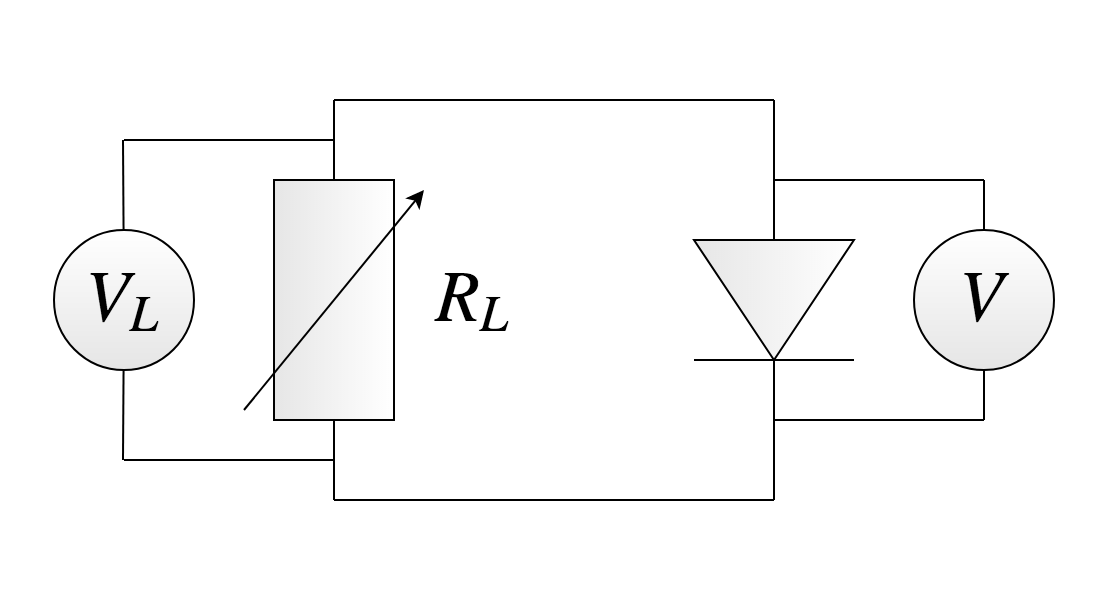
\includegraphics[scale=0.15]{krets2.png}
  \caption{Krets for å måle strøm-spenning karakteristikken til solcellen, uten en ytre påtrykket spenning.}
  \label{krets2}
\end{figure}
\subsection{Solcellens optimale belastning}
Den optimale belastningen på en solcelle vil gi mest mulig effekt fra en belyst solcelle. Effekten beregnes fra å bruke likning \eqref{effekt1}. Det må derfor gjøres målinger av spenningen over motstanden, og strømmen gjennom den. Siden det bare er en komponent i kretsen, utenom solcellen, vil alt spenningsfallet skje over denne komponenten. Dette gjør at vi kan få all informasjonen vi trenger fra å måle spenningsfallet over motstanden, og vite resistansen. Derfor trenger vi nå bare ett voltmeter i kretsen, kretsen som ble brukt er vist i figur \vref{krets3}. Målingene for å finne optimal belastning blir gjort for samme solcelle, men med to forskjellige belysninger. Den ene belysningen er at solcellen er rettet direkte mot lyskilden for å få mest mulig bestråling. Den andre belysningen er at vi roterer solcellen rundt $\SI{60}{\degree}$ slik at strømmen i kretsen, med en lav verdi for $R_L$, er halvert.
\begin{figure}[h!]
  \centering
  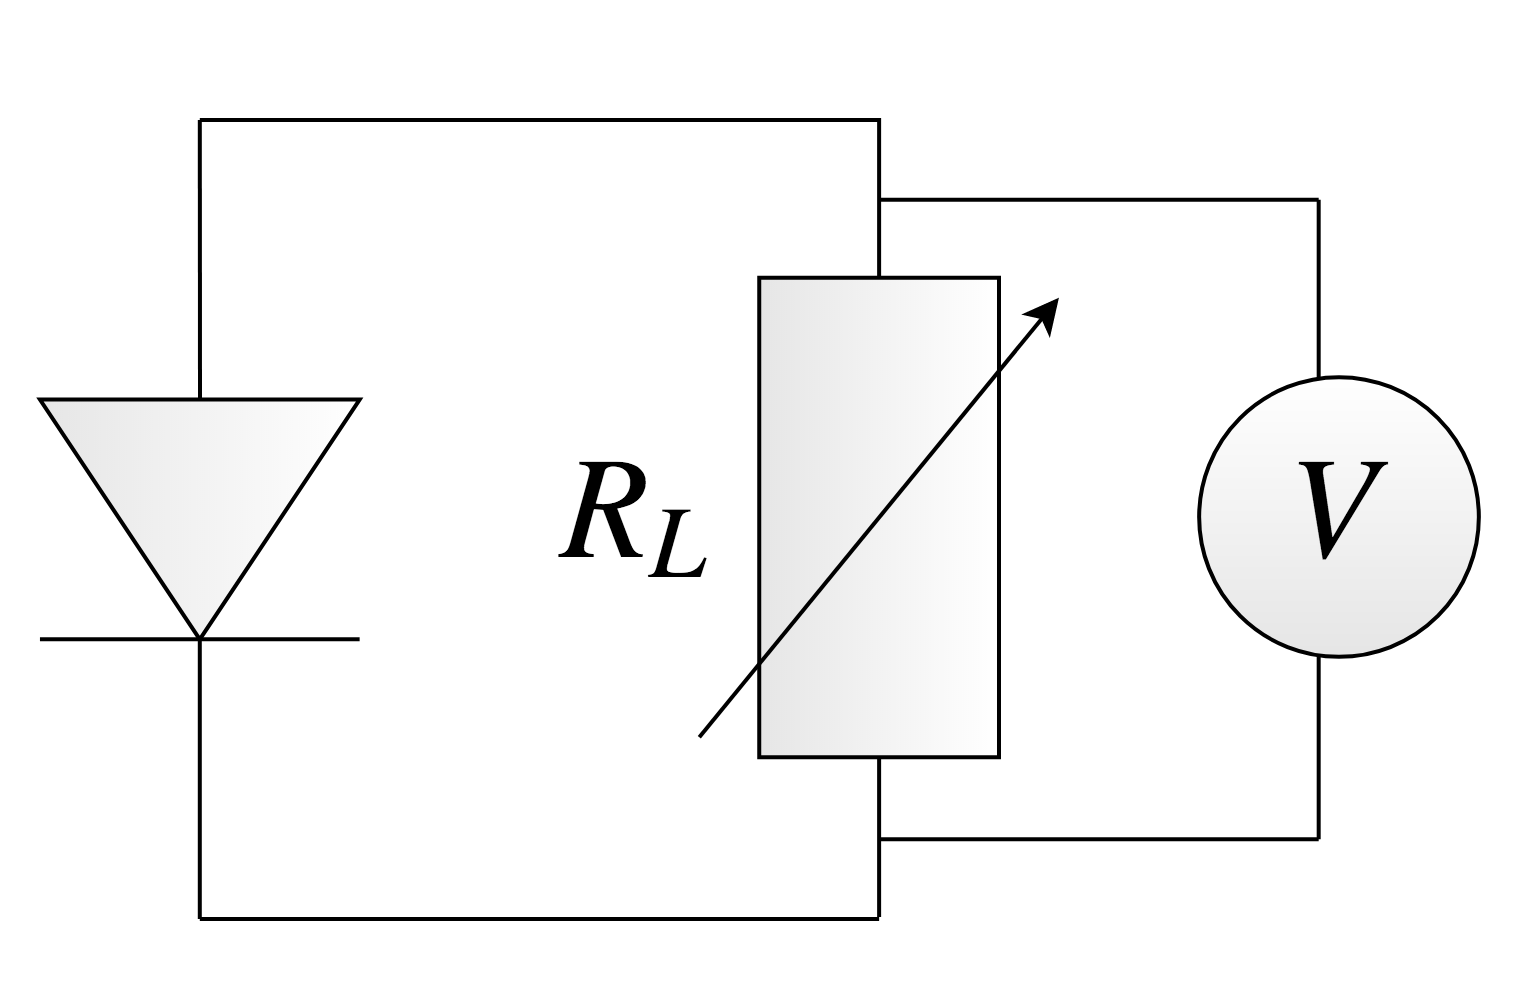
\includegraphics[scale=0.1]{krets3.png}
  \caption{Krets for å måle strøm gjennom og spenning over solcellen, for å finne den optimale belastningen til solcellen.}
  \label{krets3}
\end{figure}
\subsection{Kombinasjon av enkeltsolceller i et solcellepanel}
For å få høyere spenning fra en solcelle kobler man flere i serie, ønsker man høyere strøm kobler man dem i parallell. For å gjøre målinger på denne effekten bruker vi nå to solceller som settes i lik avstand til lyskilden. Det er to forskjellige kretser som blir brukt under målingene. En med sollcellene i parallell, og en med solcellene i serie, disse to er vist i figur \vref{krets4}. For å finne forholdet mellom den maksimale effekten for forskjellige tilfeller bruker vi likning \eqref{maxP}. Dette gjør at de to eneste egenskapene vi trenger å måle er spenningsfallet over resistansen i en åpen krets ($V_{oc}$), og strømmen i en kortsluttet krets ($I_{sc}$).
\begin{figure}[h!]
  \centering
  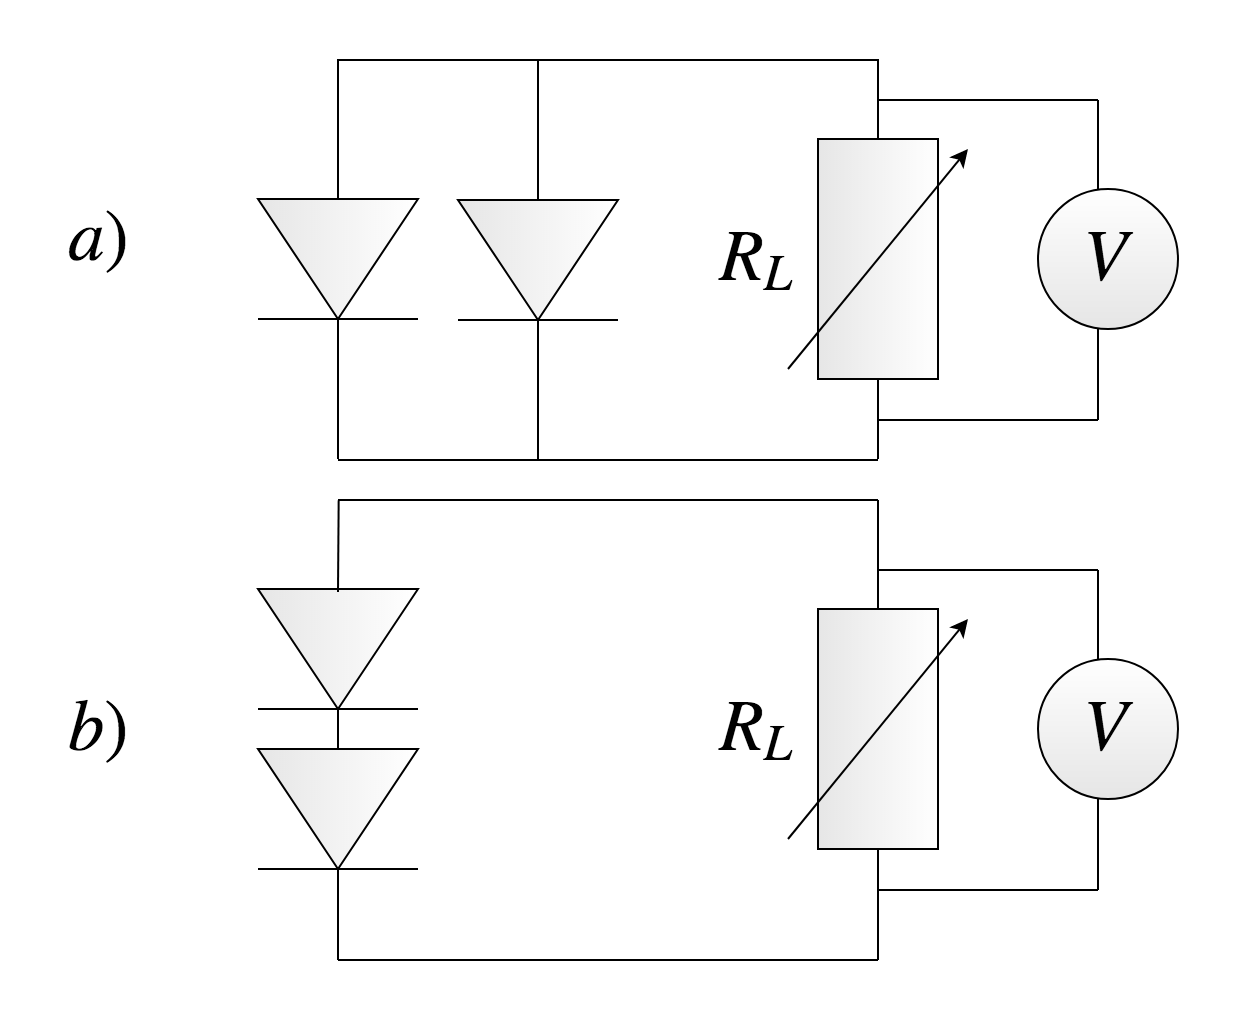
\includegraphics[scale=0.16]{krets4.png}
  \caption{Krets for å måle forskjellen i strøm og spenning når to solceller er koblet i parallell (a) iforhold til i serie (b).}
  \label{krets4}
\end{figure}
For både parallellkoblede solceller og seriekoblede solceller blir det gjort målinger av $V_{oc}$ og $I_{sc}$ for to forskjellige tilfeller. Det første tilfellet er at begge solcellene er belyst like mye. Deretter dekker vi til den ene solcellen og gjør igjen de samme målingene. Fra disse målingene kan man beregne effektivitetsforholdet mellom de to tilfellene med likning \eqref{maxP} for både serie og parallell koblede solceller.
\subsection{Solcellens effekt}
For å finne effekten til solcellen kommer vi til å bruke et solarimeter. Oppsettet under målingen av solarimeteret er vist i figur \vref{lab1}. Solarimeteret blir plassert ved samme avstand til lyskilden som solcellen, slik at strøm-spenning karakteristikken målt tidligere kan brukes. Det er to mål som må gjøres for å beregne effektiviteten til solcellen. En må måle spenningen over solarimeteret med et følsomt voltmeter, og notere seg kalibreringskonstanten til solarimeteret. Det andre en må målet er arealet til solcellen. Dette blir gjort ved å bruke et skyvelær. Grunnet formen til solcellen var det mange lengder som måtte måles. Spenningen over solarimeteret og arealet av solcellen kan brukes i likning \eqref{kalibrering} for å beregne effekten som solcellen blir belyst. Fra forholdet mellom effekten den blir belyst, og den maksimale effekten i kretsen kan vi beregne effektiviteten til solcellen med likning \eqref{effekt}.
\begin{figure}[h!]
  \centering
  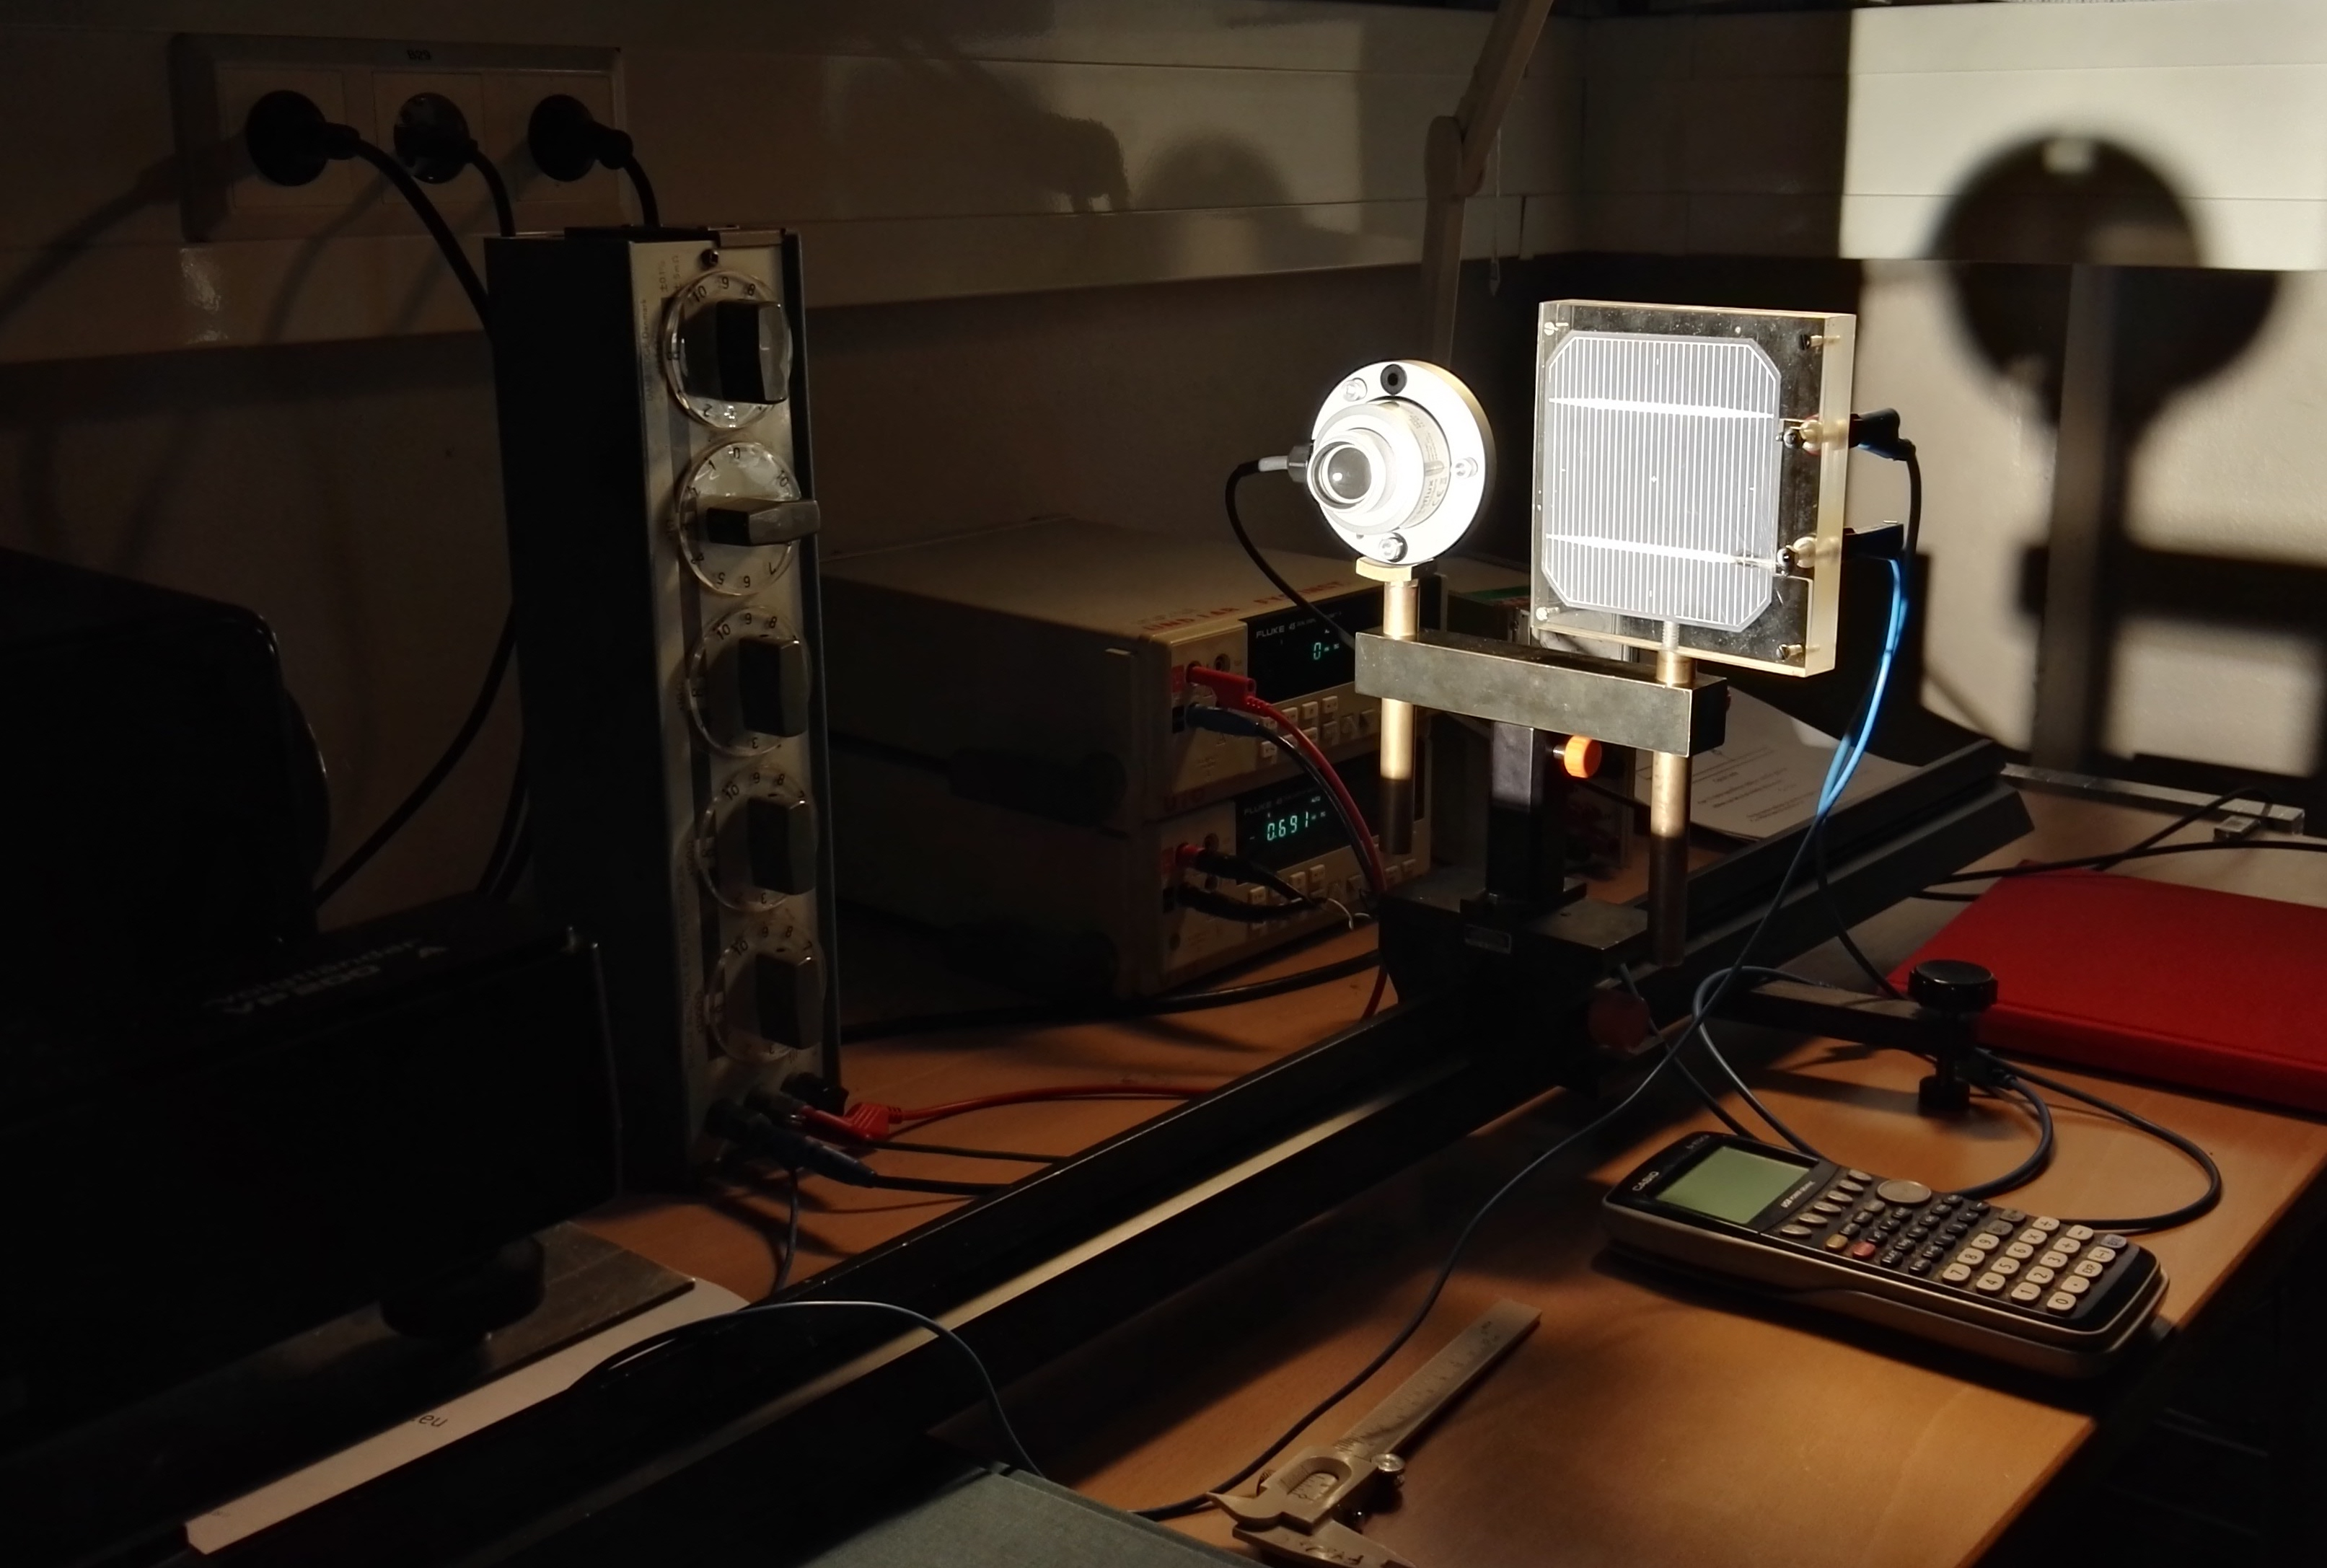
\includegraphics[scale=0.065]{lab1.jpg}
  \caption{Bilde fra laberatoriet under måling av spenningen til solarimeteret. I bildet ser vi den belyste solcellen ved siden av den belyste solarimeteret. I bakgrunnen ser vi de to multimeterene brukt under eksperimentet, og den varierende motstanden $R_L$.}
  \label{lab1}
\end{figure}
\section{Resultater}
\subsection{Strøm-spenningskarkateristikk}
For å finne strøm-spenning-spenningkarakteristikken til solcellen målte vi strømmen gjennom og spenningen over solcellen. Målingene gjort strømmen og spenningen til en belyst solcelle, med en ytre spenningskilde på $\SI{5}{\volt}$, er vist i figur \vref{resultat_ytre_spenning}. Målinger i både positiv og negativ strømretning er vist i figuren. Kretsen brukt for disse målingene er vist i figur \vref{krets1}.
\begin{figure}
  \centering
  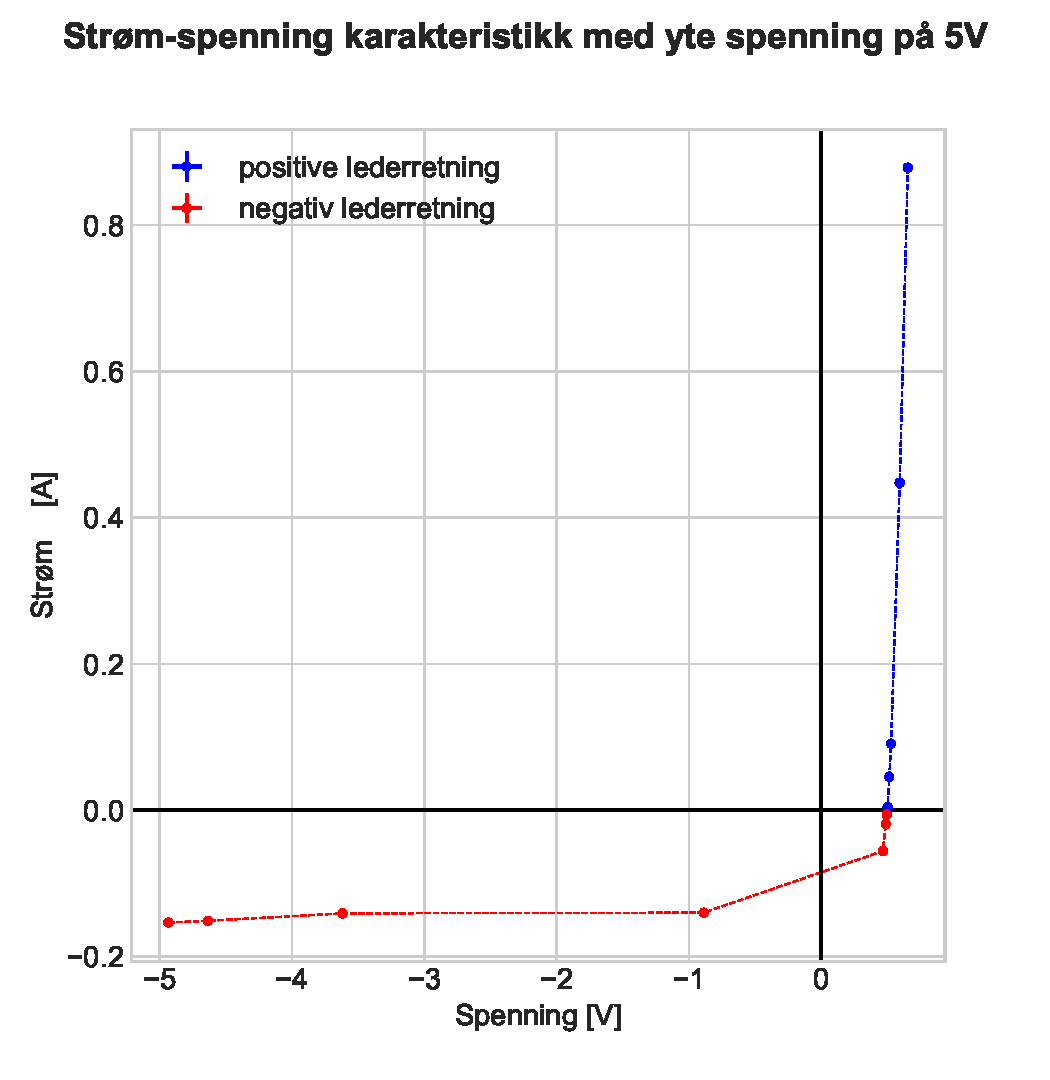
\includegraphics[scale=0.4]{ytre_spenning.pdf}
  \caption{Strøm-spenningskarkateristikken for en belyst solcelle med en ytre spenning på $5$ volt. Kretsen brukt for å gjøre disse målingene er vist i figur \vref{krets1}.}
  \label{resultat_ytre_spenning}
\end{figure}
Deretter lot vi solcellene arbeide på egenhånd, og gjorde målinger på strøm-spenningskarkateristikken uten noen ytre spenningskilde. Målingene vi gjorde er vist i figur \vref{resultat_uten_spenning}. Målingene for spenningen i en åpen krets, $V_{oc}$, og strømmen i en kortsluttet krets, $I_{sc}$, er markert i grafen. Verdien målt for $V_{oc}$ var $\SI{497.86}{\milli\volt}$, og verdien for $I_{sc}$ var $\SI{-145.821}{\milli\ampere}$.
\begin{figure}
  \centering
  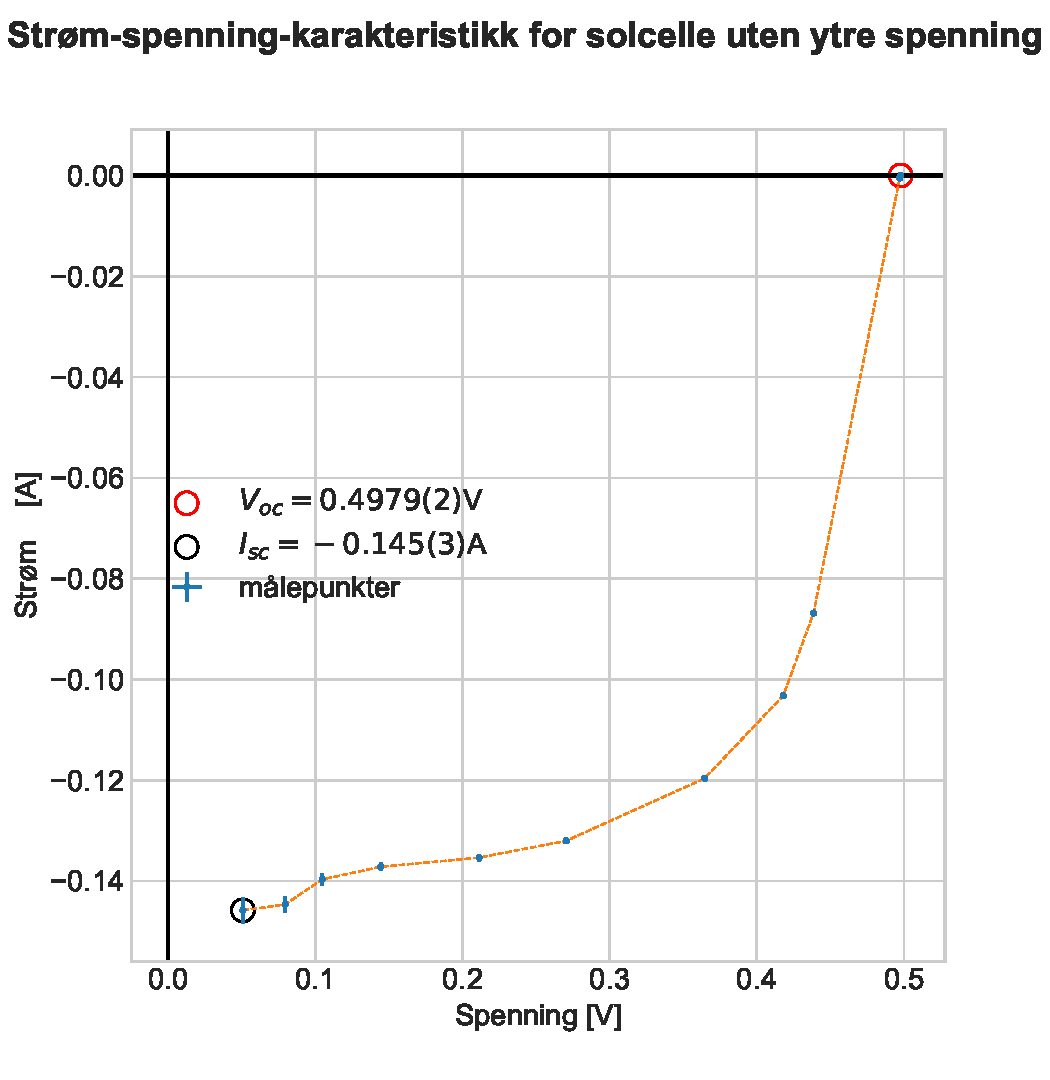
\includegraphics[scale=0.4]{strom_spenning_karr.pdf}
  \caption{Strøm-spenningskarkateristikken for en belyst solcelle uten en ytre spenningskilde. Kretsen brukt for å gjøre disse målingene er vist i figur \vref{krets2}.}
  \label{resultat_uten_spenning}
\end{figure}
\subsection{Solcellens optimale belastning}
For å finne den optimale belastningen til solcellen målte vi strømmen gjennom og spenningen over solcellen. Vi gjennbruker derfor målingene fra strøm-spenningskarkateristikken vist tidligere, itilegg til nye målinger av en redusert belyst solcelle. Resultatet fra målingene er vist i figur \vref{maling_optimal_belast}. Den redusert belyste solcellen i figuren er dreid omlag $60\degree$ vekk fra lyskilden, dette resultert i omtrent halvert strøm for en lav resistanse $\approx 0.5\Omega$.
\begin{figure}
  \centering
  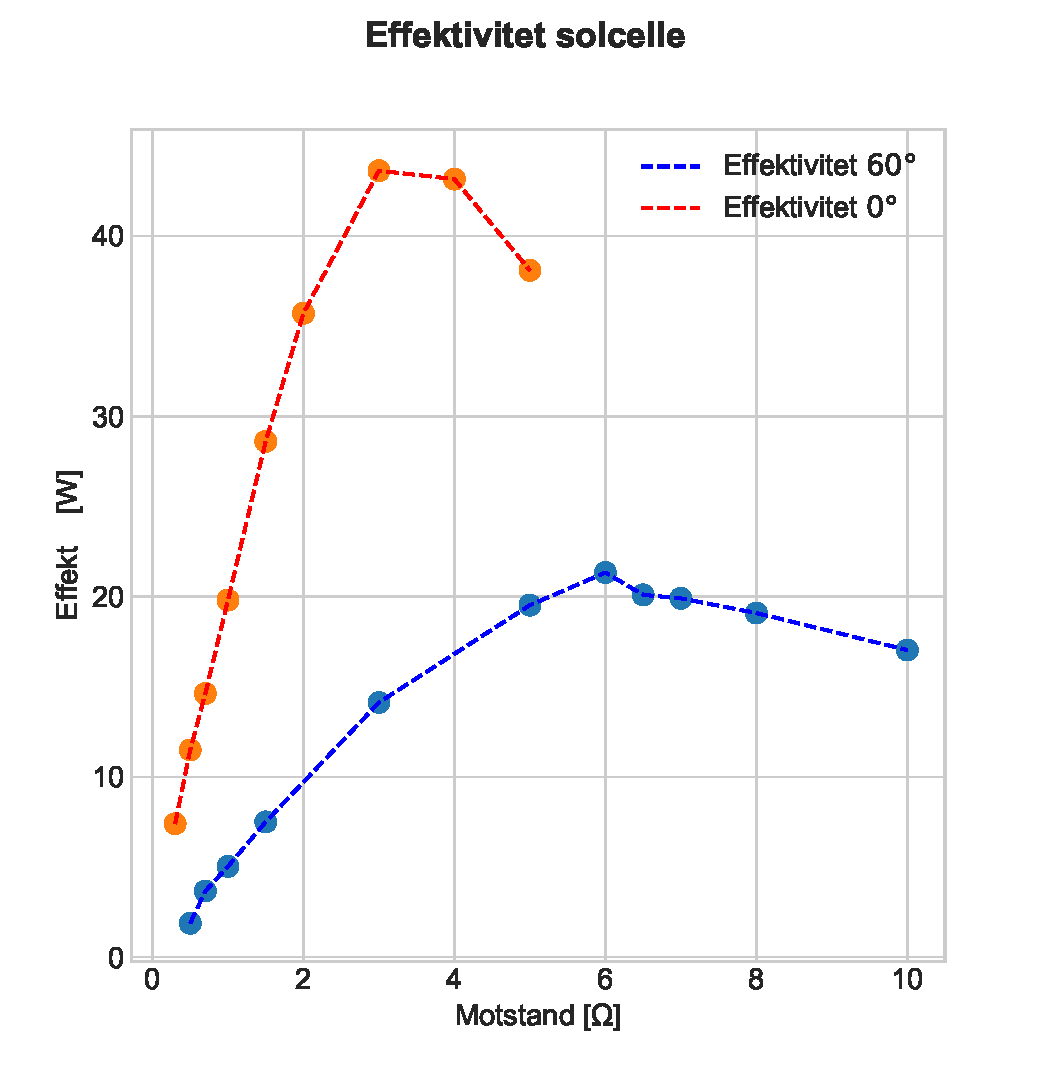
\includegraphics[scale=0.4]{effekt.pdf}
  \caption{Effekten til solcellen som en funksjon av motstanden i kretsen. Det røde datasettet er med en solcelle som er optimalt belyst, og det blå er for en solcelle som er rotert $60\degree$ vekk fra lyskilden.}
  \label{maling_optimal_belast}
\end{figure}
Målingene viser at man får en større effekt fra solcellen om de er rettet mot lyskilden. Solcellen klarer å få en effekt på $\SI{43.615}{\watt}$ når motstandslasten er på $\SI{3}{\Omega}$. For solcellen som er vendt $60\degree$ vekk fra lyskilden gir en maksimal effekt på $\SI{21.33}{\watt}$ med en motstand på $\SI{6}{\Omega}$.
\newpage
\subsection{Kombinasjon av enkeltsolceller i et solcellepanel}
Ved denne målingen ønsker vi å finne forholdet mellom maksimal effekt for solceller under forskjellige koblinger og lysforhold. Fra å måle strømmen i en sluttet krets, og spenningen i en åpen krets, kan man finne forholdet mellom effekten i kretsen ved å bruke likning \eqref{maxP}. Vi gjorde derfor målinger på de to verdiene med solcellene koblet i paralell, og serie, med begge belyst, og med en belyst. Resulatene fra disse målingene er vist i tabell \vref{effekt2}.
\begin{table}[h]
\renewcommand\arraystretch{1.3}
\begin{adjustwidth}{-0.3in}{0.1in}
\begin{tabular}{|l | *{3}{>{\centering}p{2cm}|}c|}
\hline Kobling & \multicolumn{2}{c|}{Serie} & \multicolumn{2}{c|}{Parallell} \\
\hline Måling & $V_{oc}$[mV]    &   $I_{sc}$ [mA]  &   $V_{oc}$ [mV]  &  \,\,\,\,\,\,$I_{sc}$ [mA]\,\,\,\,\,\, \\
\hline Begge belyst & -499.82    &   -293.20  &   -1000.87  &  -139.62\\
\hline En belyst    & -461.53    &   -155.17  &   -634.704  &  -427.60\\ \hline
\end{tabular}
\end{adjustwidth}
\caption{Målinger gjort av spenningen i en åpen krets, og strømmen i en kortsluttet krets. Fra disse verdiene kan vi beregne forholdet mellom effektiviteten til de forskjellige tilfellene.}
\label{effekt2}
\end{table}
Fra å bruke likning \eqref{maxP} på dataen vist i tabell \vref{effekt2} kan en beregne fram til informasjon om de relative effektene for forskjellige koblinger og lysforhold. Når vi har begge solcellene belyst får vi rundt $5\%$ mer effekt fra å ha solcellene i serie iforhold til i parallell. Derimot hvis bare en av solcellene er belyst får vi en faktor $3.79$ mer effekt fra å ha solcellene i parallell iforhold til å ha solcellene i seriekobling. For solceller koblet i serier viser det seg at forholdet mellom én belyst og begge belyst er en faktor $2.05$ mer effekt fra at begge er belyst iforhold til bare en belyst. Det samme forholdet gjelder for solceller i parallell, men motsatt vei, for parallell kobling får man en faktor $1.94$ mer effekt fra å ha én solcellene belyst iforhold til begge.
\subsection{Solcellens effektivitet}
Ved å plasere et solarimeter ved samme avstand til lyskilden som solcellen kan man beregne effektiviteten til solcellen. Solarimeteret som ble brukt under eksperimentet hadde kalibreringskonstant $a=\SI{11.13}{\micro\volt\meter^2\per\watt}$. Ved å bruke et skyvelær for å måle de forskjellige geometriske størrelsene til solcellen fant vi at arealet til solcellen var $\SI{96.27}{\centi\meter^2}$. Gjennomsnittet av flere målinger til spenningen over solarimeteret viste seg å være $\SI{686.2}{\milli\volt}$. Med disse målingene kan man bruke likning \eqref{kalibrering} til å vise at den innstråle effekten er
$\SI{593.54}{\watt}$. Denne verdien, sammen med den maksimale effekten som har blitt målt fra solcellen, som vist i figur \vref{maling_optimal_belast}, er $\SI{43.615}{\watt}$, kan vi beregne effekten til solcellen med likning \eqref{effekt}. Vi finner at effekten til solcellen er $7.35\%$.
\section{Diskusjon}
\subsection{Strøm-spenningkarakteristikk}
Målingen av strøm-spenningkarakteristikk ble gjort med og uten en ytre spenningskilde. Fra å se på målingene med en ytre spenningskilde, vist i figur \vref{resultat_ytre_spenning}, kan man se en viktig egenskap med solceller. Solceller leder strøm i en retning, men ikke i en annen. Solcellen oppfører seg som en diode. Når strømmen går i positiv lederretningen har vi et positivt spenningsfall over solcellen, og positiv strøm i kretsen. Forholdet mellom strømmen og spenningsfallet ser ut til å øke eksponesielt. Av å snu polariteten på spenningskilden fikk vi målinger av strøm-spenningkarakteristikk i negativ lederrtening. Disse målepunktene sier oss at strømmen i kretsen går fort mot en lav og konstant verdi, som er uavhengig av spenningen over solcellen, når strømmen beveger seg i sperreretning. Når motstanden er minst skjer all spenningsfallet over solcellen, for høyere motstander nærmer strømmen i kretsen seg $0$, men går aldri over på grunn av polariteten på spenningskilden.\par
Målingene gjort av strøm-spenningskarkateristikken uten en ytre spenningskilde er vist i figur \vref{resultat_uten_spenning}. Kurven på grafen er slik en forventer for en belyst solcelle. Formen på kurven er lik karakteristikken med en ytre spenningskilde. For lave resistanser flater strømmen ut mot en konstant verdi, som går mot $I_{sc}$. For høyere motstander øker strømmen eksponensielt, og skjærer $x$-aksen i $V_{oc}$ hvor kretsen er åpen, det vil si uendlig motstand. Den maksimale spenningen fra en enkelt solcelle går mot $\SI{0.5}{\volt}$. Av å bestemme den maksimale effekten til solcellen finner en det største arealet mulig innenfor kurven i den fjerde kvadrant.
\subsection{Solcellens effektivitet}
Fra å se på grafen vist i figur \vref{maling_optimal_belast} er det to ting å merke seg. Den første, og den mest naturlige, er at solcellen som blir mer belyst gir en større effekt. Den andre er at hvilken lastmotstand som resulterer i maksimale effekten avhenger av bestrålingen. For den fullt belyste solcellen er resistansen som resulterer i størst effekt $\SI{3}{\Omega}$, for den redusert belyste er resistansen $\SI{6}{\Omega}$. Dette er et viktig faktum ved solceller. Ønsker du størst mulig effekt fra solcellen burde lasten i kretsen variere med belysningen av solcellen. Den maksimale effektforskjellen er omtrent en faktor to forskjellig mellom den fullt og redusert belyste solcellen.
\subsection{Kombinasjon av enkeltsolceller i et solcellepanel}
Fra målingen vist i tabell \vref{effekt2} er det lett å se at det å koble flere solceller i parallell øker spenningen i kretsen, og koble solceller i serie øker strømmen. Begge disse egenskapen vil dobbles iforhold til den den andre koblingen. Fra tabellen kan en også se effekten av å bestråle to solceller iforhold til en, og hvordan koblingsmåte påvirker dette. For seriekobling halveres strømmen, men spenningen er nesten uforandret, når det blir belyst en solcelle istedenfor to. For parallellkobling synker både strøm og spenning. Spenningen blir litt under halvert, og strømmen er en faktor tre svakere.\par
Ved å bruke likning \eqref{maxP} kan en beregne forholdet mellom effekten for de forskjellige tilfellene. Det er da viktig å huske på at denne likningen er en tilnærming. Fill factor antas å være en karakteristikk ved solcellen som ikke er avhengig av ytre forhold. Dette gjør at den er tilnærmet konstant, og denne tilnærmingen skaper en usikkerhet i forholdet mellom effektene. En ville fått en mer nøyaktig verdi for effekten ved å måle strøm-spenningkarakteristikken for solcellene under alle forholdene. Dette ble ikke gjort under eksperimentet fordi det ville vært mer tidkrevene. Fra å se på forholdet mellom effektene for de ulike koblingene og lysforholdene kan en gjøre flere slutninger om hvordan en kan jeg gjøre solceller mest effektive. Når to solceller er i parallell, men den ene er ubelyst, får man nesten fire ganger så mye effekt fra å ha solcellene i parallell iforhold til å dem koblet i serie. Årsaken til dette er at solceller oppfører seg som en diode når de ubelyst. Derfor vil kretsen kortsluttes når kunn den ene solcellen er belyst. For en parallellkobling vil dette ikke føre til at kretsen blir kortsluttet, siden den belyste solcellens påvirkning i kretsen ikke vil bli påvirket av den andre solcellen.
\subsection{Solcellens effekt}
Under beregning av arealet tok vi hensyn til formen på solcellen, som en ser i figur \vref{lab1}, men vi tok ikke hensyn til fingrene på tverrs av solcellen. Årsaken til dette er at 
%\subsubsection*{Utstyrsliste}
%\begin{itemize}
%\label{utstyr}
%\item meterstokk - Hultafors
%\end{itemize}
\begin{thebibliography}{9}
\bibitem{squires}
Squires, G.L. \emph{Practical Physics}, Cambridge University Press, 2001.
\bibitem{oppgave}
Fysisk institutt, \emph{FYS 2150. SOLCELLEN}, Univseritet i Oslo, februar 2017.
\end{thebibliography}
\end{document}
